% !TEX program = xelatex
\documentclass[11pt]{beamer}

%%%%%%%%%%%%%%%%%%%%%%%%%%%%%%%%%%%%%%%%%%%%%%%%%%%%
% Metropolis
\usepackage{FiraSans}
\setsansfont[BoldFont={Fira Sans SemiBold}]{Fira Sans Book}

\usetheme[progressbar=frametitle]{metropolis}
% For customization, see: http://ctan.mackichan.com/macros/latex/contrib/beamer-contrib/themes/metropolis/doc/metropolistheme.pdf

% For tikz plotting
%\usepackage{tikz}
%\usetikzlibrary(positioning)
%\usepackage{pgfplots}

%Uncomment for "blank" theme
\definecolor{osugray}{HTML}{5c5c5c}
\setbeamercolor{frametitle}{fg=black, bg=black!2}
\setbeamercolor{title}{fg=black}
\setbeamercolor{title separator}{fg=black}
\setbeamercolor{progress bar}{fg=osugray, bg=black!2}
\setbeamercolor{author}{fg = black}
\setbeamercolor{normal text}{fg = black}


%Uncomment for OSU theme
%\definecolor{osured}{RGB}{187,0,0}
%\definecolor{darkscarlett}{RGB}{131,0,0}
%\definecolor{osugray}{HTML}{5c5c5c}
%\definecolor{osublue}{HTML}{1e5357}
%\setbeamercolor{frametitle}{bg=darkscarlett}
%\setbeamercolor{title}{fg=osured}
%\setbeamercolor{title separator}{fg=osugray}
%\setbeamercolor{progress bar}{fg=osugray, bg=black!2}
%\setbeamercolor{normal text}{fg = black}
%%%%%%%%%%%%%%%%%%%%%%%%%%%%%%%%%%%%%%%%%%%%%%%%%%%%%%%%%%%%%%%

% Tikz
\usepackage{tikz}
\usepackage{xcolor}

\usepackage{pgfplots}
\usepackage{xspace}
\newcommand{\themename}{\textbf{\textsc{metropolis}}\xspace}

\usepackage{natbib}

\usepackage{mathtools,amsmath}

% Table
\usepackage{graphicx}% http://ctan.org/pkg/graphicx
\usepackage{subfig} % side-by-side pgfplots
\usepackage{multirow}




%=======%
% Title %
%=======%

\title{\large{Unexpected Contributions in Wartime Coalitions}}

\author{J. Andres Gannon\textsuperscript{1} \\
  Daniel Kent\textsuperscript{2}}

\institute{\textsuperscript{1} University of California, San Diego,
  \textit{jagannon@ucsd.edu} \\
\textsuperscript{2} The Ohio State University,
\textit{kent.249@osu.edu}}

\date{}
% logo of my university

%\titlegraphic{\tikz\node[opacity = 0.2]{\includegraphics[scale = 0.75]{OSU_logo.jpg}};}

\begin{document}


\begin{frame}
  \titlepage
\end{frame}

\begin{frame}{Overview}
  A few empirical areas to look out for:
  \begin{itemize}
    \item Does structural equivalence make sense for tie strength?
    \item How to deal with the Canada outlier?
    \item Is use of GAMs convincing?
  \end{itemize}
\end{frame}

\begin{frame}{Puzzle}
	\begin{itemize}
		\item Why do some countries punch above their weight when contributing to coalition conflicts?
  \end{itemize}
\begin{table}[]
\begin{tabular}{lll}
\hline
\textbf{Year} & \textbf{Country}  & \textbf{Percent} \\ \hline
2001          & Denmark           & 0.66             \\
2001          & New Zealand       & 0.65             \\
2001          & United States     & 0.53             \\
2001          & Romania           & 0.53             \\
2001          & Netherlands       & 0.44             \\
2001          & Germany           & 0.44             \\
2001          & Norway            & 0.34             \\
2001          & Australia         & 0.29             \\
2001          & Turkey            & 0.27             \\
2001          & Spain             & 0.20             \\ \hline
\end{tabular}
\end{table}
\end{frame}


\begin{frame}{Theory}
  \begin{figure}[H]
		\centering
		\begin{tikzpicture}
		% Graph axes
		\draw[thick,<->] (0,5) node[above]{Expected Cost} -- (0,0) -- (8,0) node[right]{Tie Strength};

		% Contribution Curve
		\draw[thick] (0,0)..controls (5,5) ..(8,2.5);

		% Desired Relationship Tie
		\draw[dashed] (4,0) -- (4,3.5);
		\draw[dashed] (6.5,0) -- (6.5,3.5);
		\draw[decorate,decoration={brace,mirror,raise=5pt}, thick]
		(4,0) -- (6.5,0);
		\node at (5.25,-0.7) {Desire Improved Tie};
		\end{tikzpicture}
    \label{fig:theory}
  \end{figure}
\end{frame}


\begin{frame}{Point}
Outsized contributions signal a desire for a stronger relationship \textit{and} reliability as a future partner.

\begin{itemize}
  \item Costly transmission of information
  \item Anticipate future payoffs because of reputation and reciprocity
\end{itemize}

\end{frame}

\begin{frame}{Goal is to convince you that...}
Theories of alliance contributions incorrectly focus on:

\begin{itemize}
  \item \textit{Current} alliance tie, not \textit{desired}
  \item \textit{Value} of contribution, not \textit{cost}
\end{itemize}

We can explain contributions to the Afghanistan War (ISAF), particularly over-contributions, better through desired ties better than existing theories.

\end{frame}

\begin{frame}{Problems with conventional explanations}
  Largest share of forces are contributed by:
  \begin{enumerate}
    \item Collective action (Olsen and Zeckhauser 1966) -- powerful states
    \item Balance of threat (Walt 19870) -- most threatened states
    \item Alliance politics (Snyder 1984) -- closest friends
    \item Domestic politics (Ashraf 2011) -- consistency with political ideology
  \end{enumerate}
\end{frame}

\begin{frame}{Problems with conventional explanations}
  Largest share of forces are contributed by:
  \begin{enumerate}
    \item Collective action (Olsen and Zeckhauser 1966) -- powerful states
      \begin{itemize}
        \item Many expected free-riders don't
      \end{itemize}
    \item Balance of threat (Walt 19870) -- most threatened states
      \begin{itemize}
        \item Non-threatened states make large contributions
      \end{itemize}
    \item Alliance politics (Snyder 1984) -- closest friends
      \begin{itemize}
        \item Closest friends don't over-exert
      \end{itemize}
    \item Domestic politics (Ashraf 2011) -- consistency with political ideology
      \begin{itemize}
        \item Extent of contribution unexplained
      \end{itemize}
  \end{enumerate}
\end{frame}

\begin{frame}{We instead look at:}
  \begin{itemize}
    \item Which states carry the highest burden in US-led operations
    \item Which states most desired improved ties with the US
  \end{itemize}
\end{frame}

\begin{frame}
  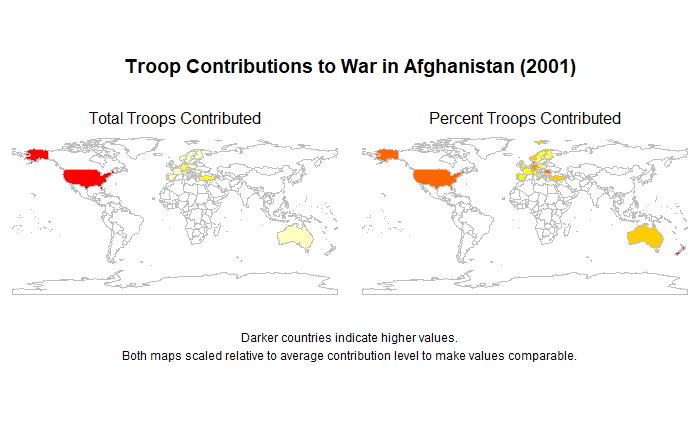
\includegraphics[scale = 0.45]{troops_2001_sidebyside_scaled.png}
\end{frame}


\begin{frame}{Theory}
  States wanting a closer relationship with the United States will make higher cost contributions to US-led war efforts

  \begin{itemize}
    \item \textbf{DV: Higher cost contribution} -- larger strain on armed forces
    \item \textbf{IV: Desire for closer relationship} -- ``acquaintances'' wanting to become ``best friends''
  \end{itemize}
\end{frame}

\begin{frame}{Theory}
  States wanting a closer relationship with the United States will make higher cost contributions to US-led war efforts

  They are a costly signal of desiring a stronger relationship:
  \begin{itemize}
    \item Benefit to US without immediate benefit to over contributor
    \item Cost to over-contributor (resource strain, risk of casualties/collateral damage)
  \end{itemize}

  Which creates:
  \begin{itemize}
    \item Reputation of reliability
    \item Expectation of reciprocity
  \end{itemize}
\end{frame}

\begin{frame}{Data}
\textbf{\underline{Unit of Analysis}}:

Country-year (2001-2005)

Troop contributions:
\begin{itemize}
  \item Binary (commit or not)
  \item Ratio of available forces
\end{itemize}

\end{frame}

\begin{frame}{Empirical Data -- 2001}
Top 10 Contributors
\quad
\quad
\quad
\quad
\quad
\quad
\;
Bottom 10 Contributors \\
\begin{tabular}{ll}
\hline
\textbf{Country} & \textbf{Percent} \\ \hline
Denmark          & 0.66             \\
New Zealand      & 0.65             \\
United States    & 0.53             \\
Romania          & 0.53             \\
Netherlands      & 0.44             \\
Germany          & 0.44             \\
Norway           & 0.34             \\
Australia        & 0.29             \\
Turkey           & 0.27             \\
Spain            & 0.20             \\ \hline
\end{tabular}
\quad
\quad
\quad
\;
\begin{tabular}{ll}
\hline
\textbf{Country} & \textbf{Percent} \\ \hline
Finland          & 0.14             \\
Austria          & 0.13             \\
Sweden           & 0.12             \\
Albania          & 0.11             \\
Greece           & 0.07             \\
Poland           & 0.05             \\
Belgium          & 0.05             \\
Bulgaria         & 0.04             \\
Portugal         & 0.02             \\
Czech Republic   & 0.01             \\ \hline
\end{tabular}
\end{frame}

\begin{frame}{Model}
  \begin{itemize}
    \item Who contributes any troops?
    \item Among contributors, what percent of available troops does each country provide?
  \end{itemize}

  \begin{align*}
    Contribution \sim f(& tie\_strength \; + \; ideological\_distance \; + \\
                        & physical\_distance \; + \;  democracy)
  \end{align*}

\end{frame}


\begin{frame}{}
  \centering
  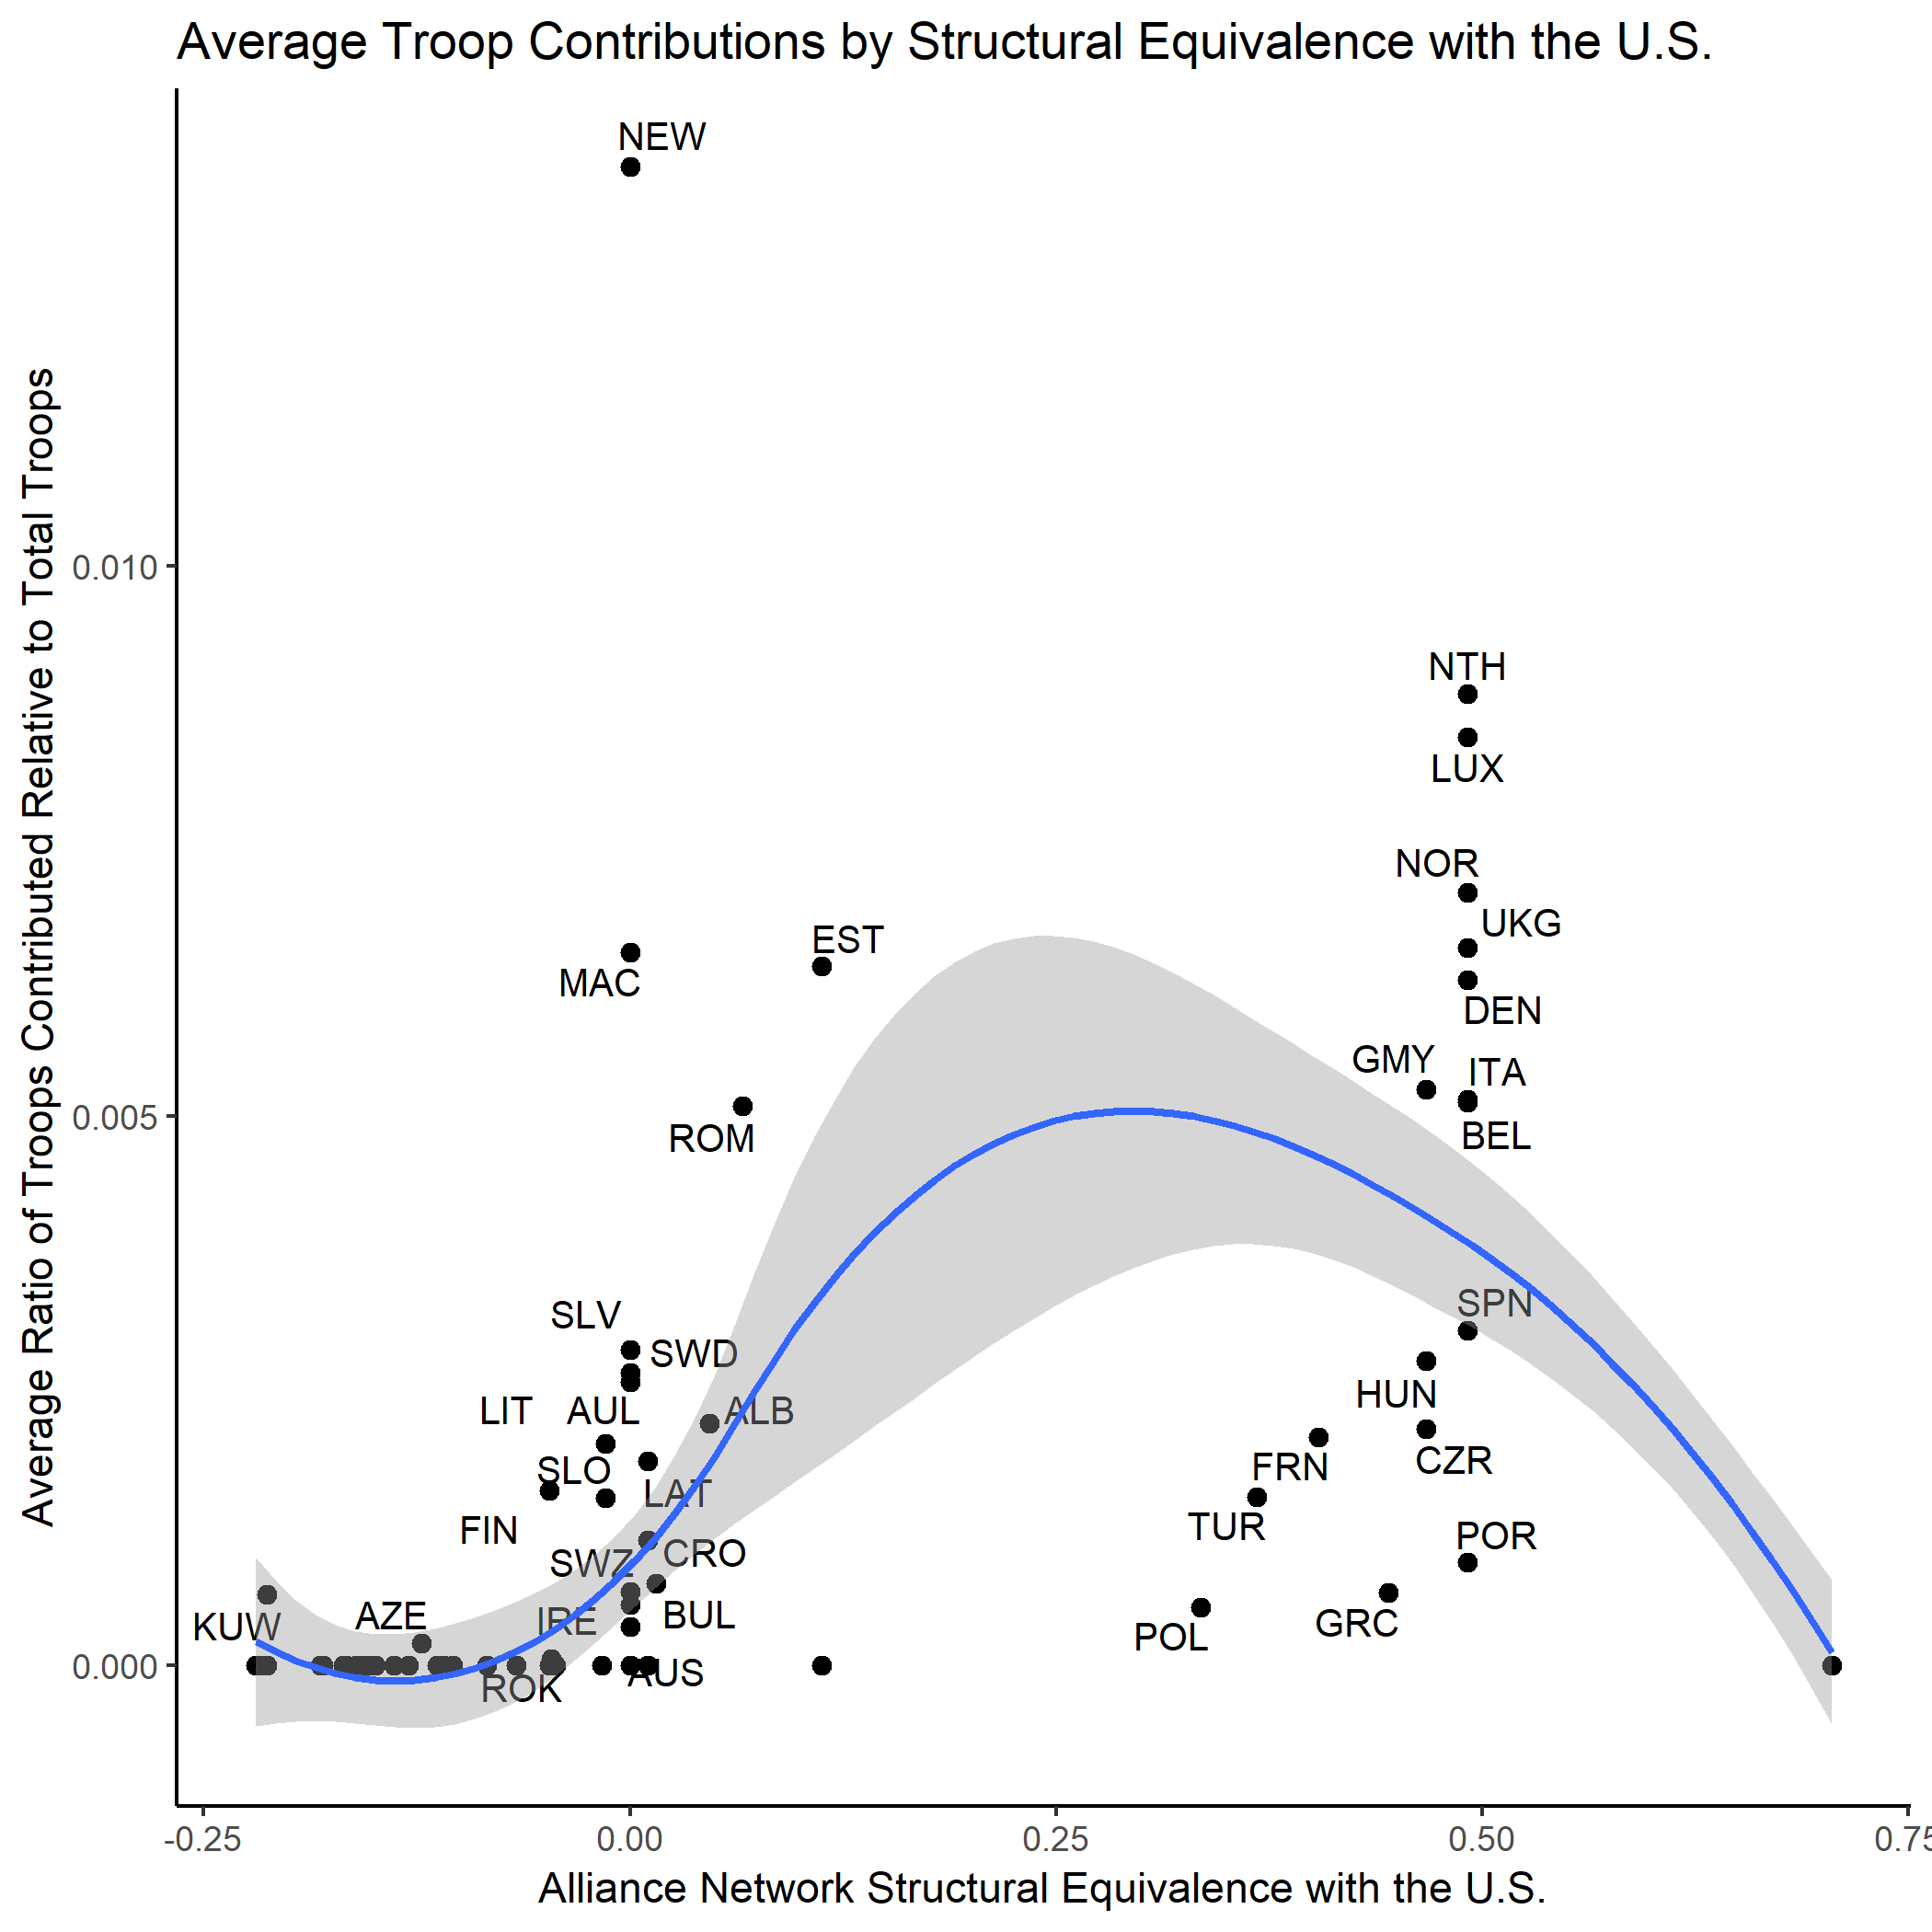
\includegraphics[scale = 0.575]{../figures/contributions.png}
\end{frame}

\begin{frame}{}
  \centering
  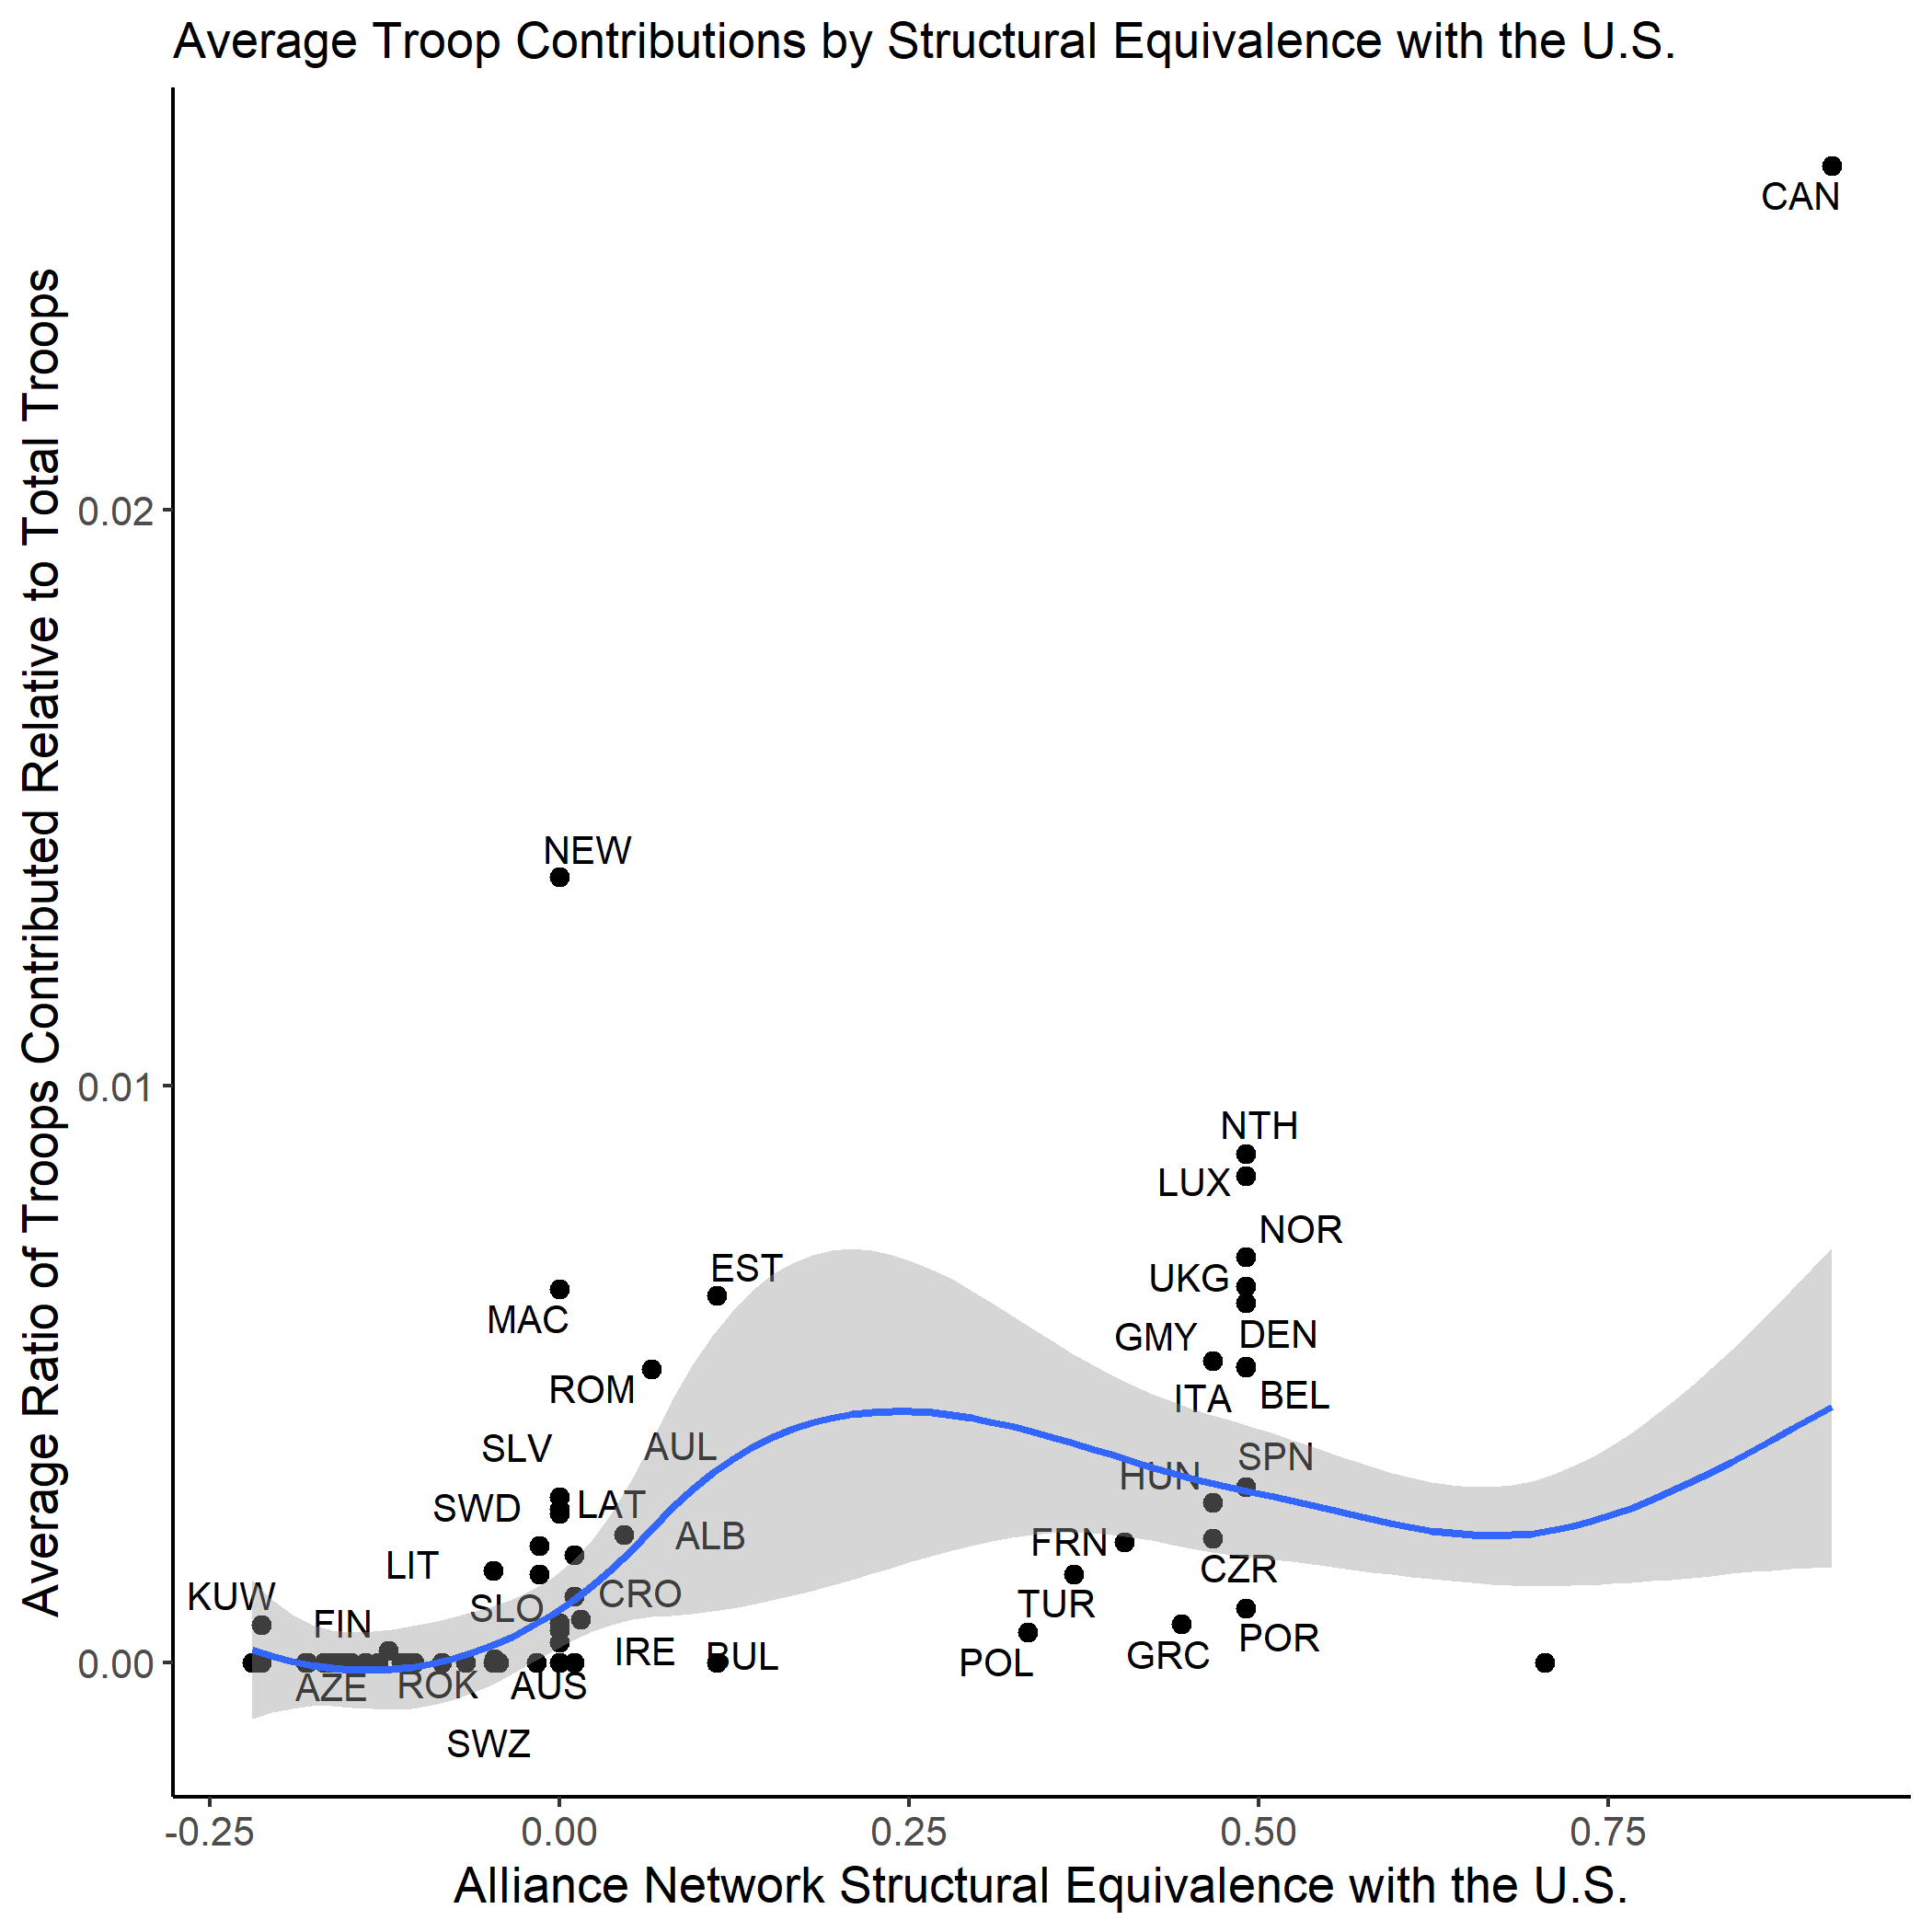
\includegraphics[scale = 0.55]{../figures/contributions_canada.png}
\end{frame}

\begin{frame}{Who Contributes?}
  \centering
  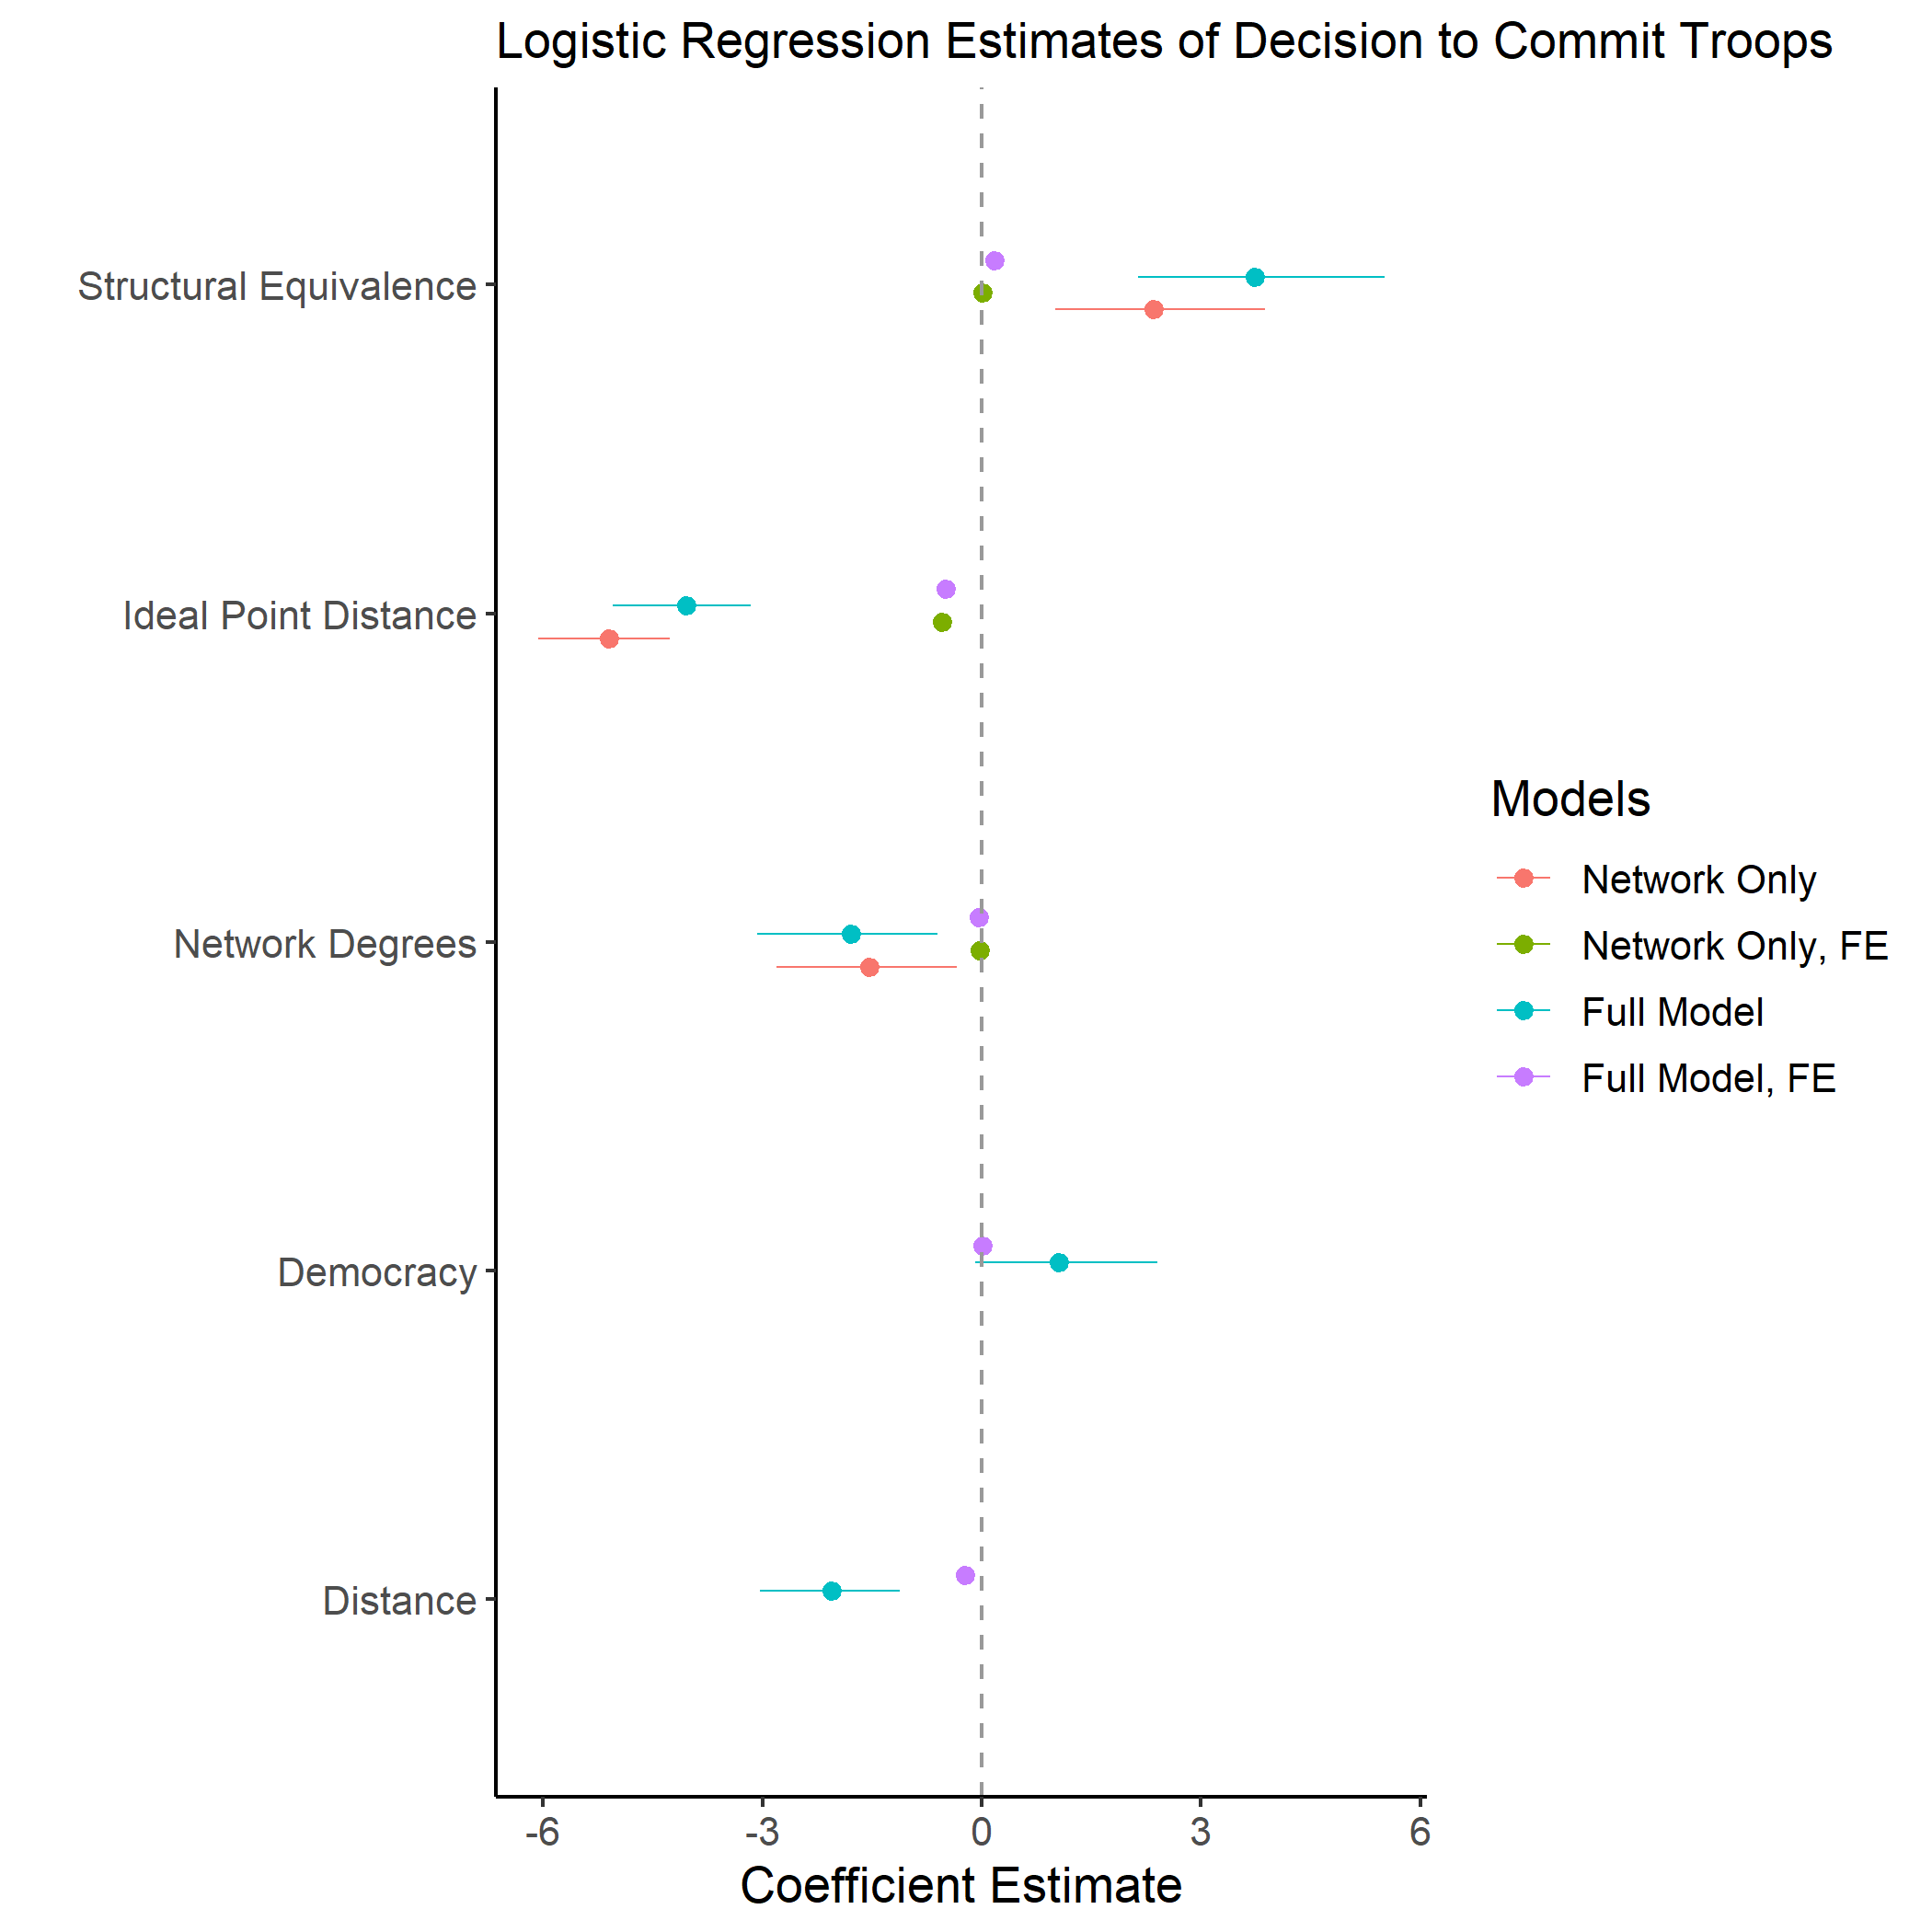
\includegraphics[scale=0.45]{../figures/logit_coef.png}
\end{frame}

\begin{frame}{Who Contributes?}
  \centering
  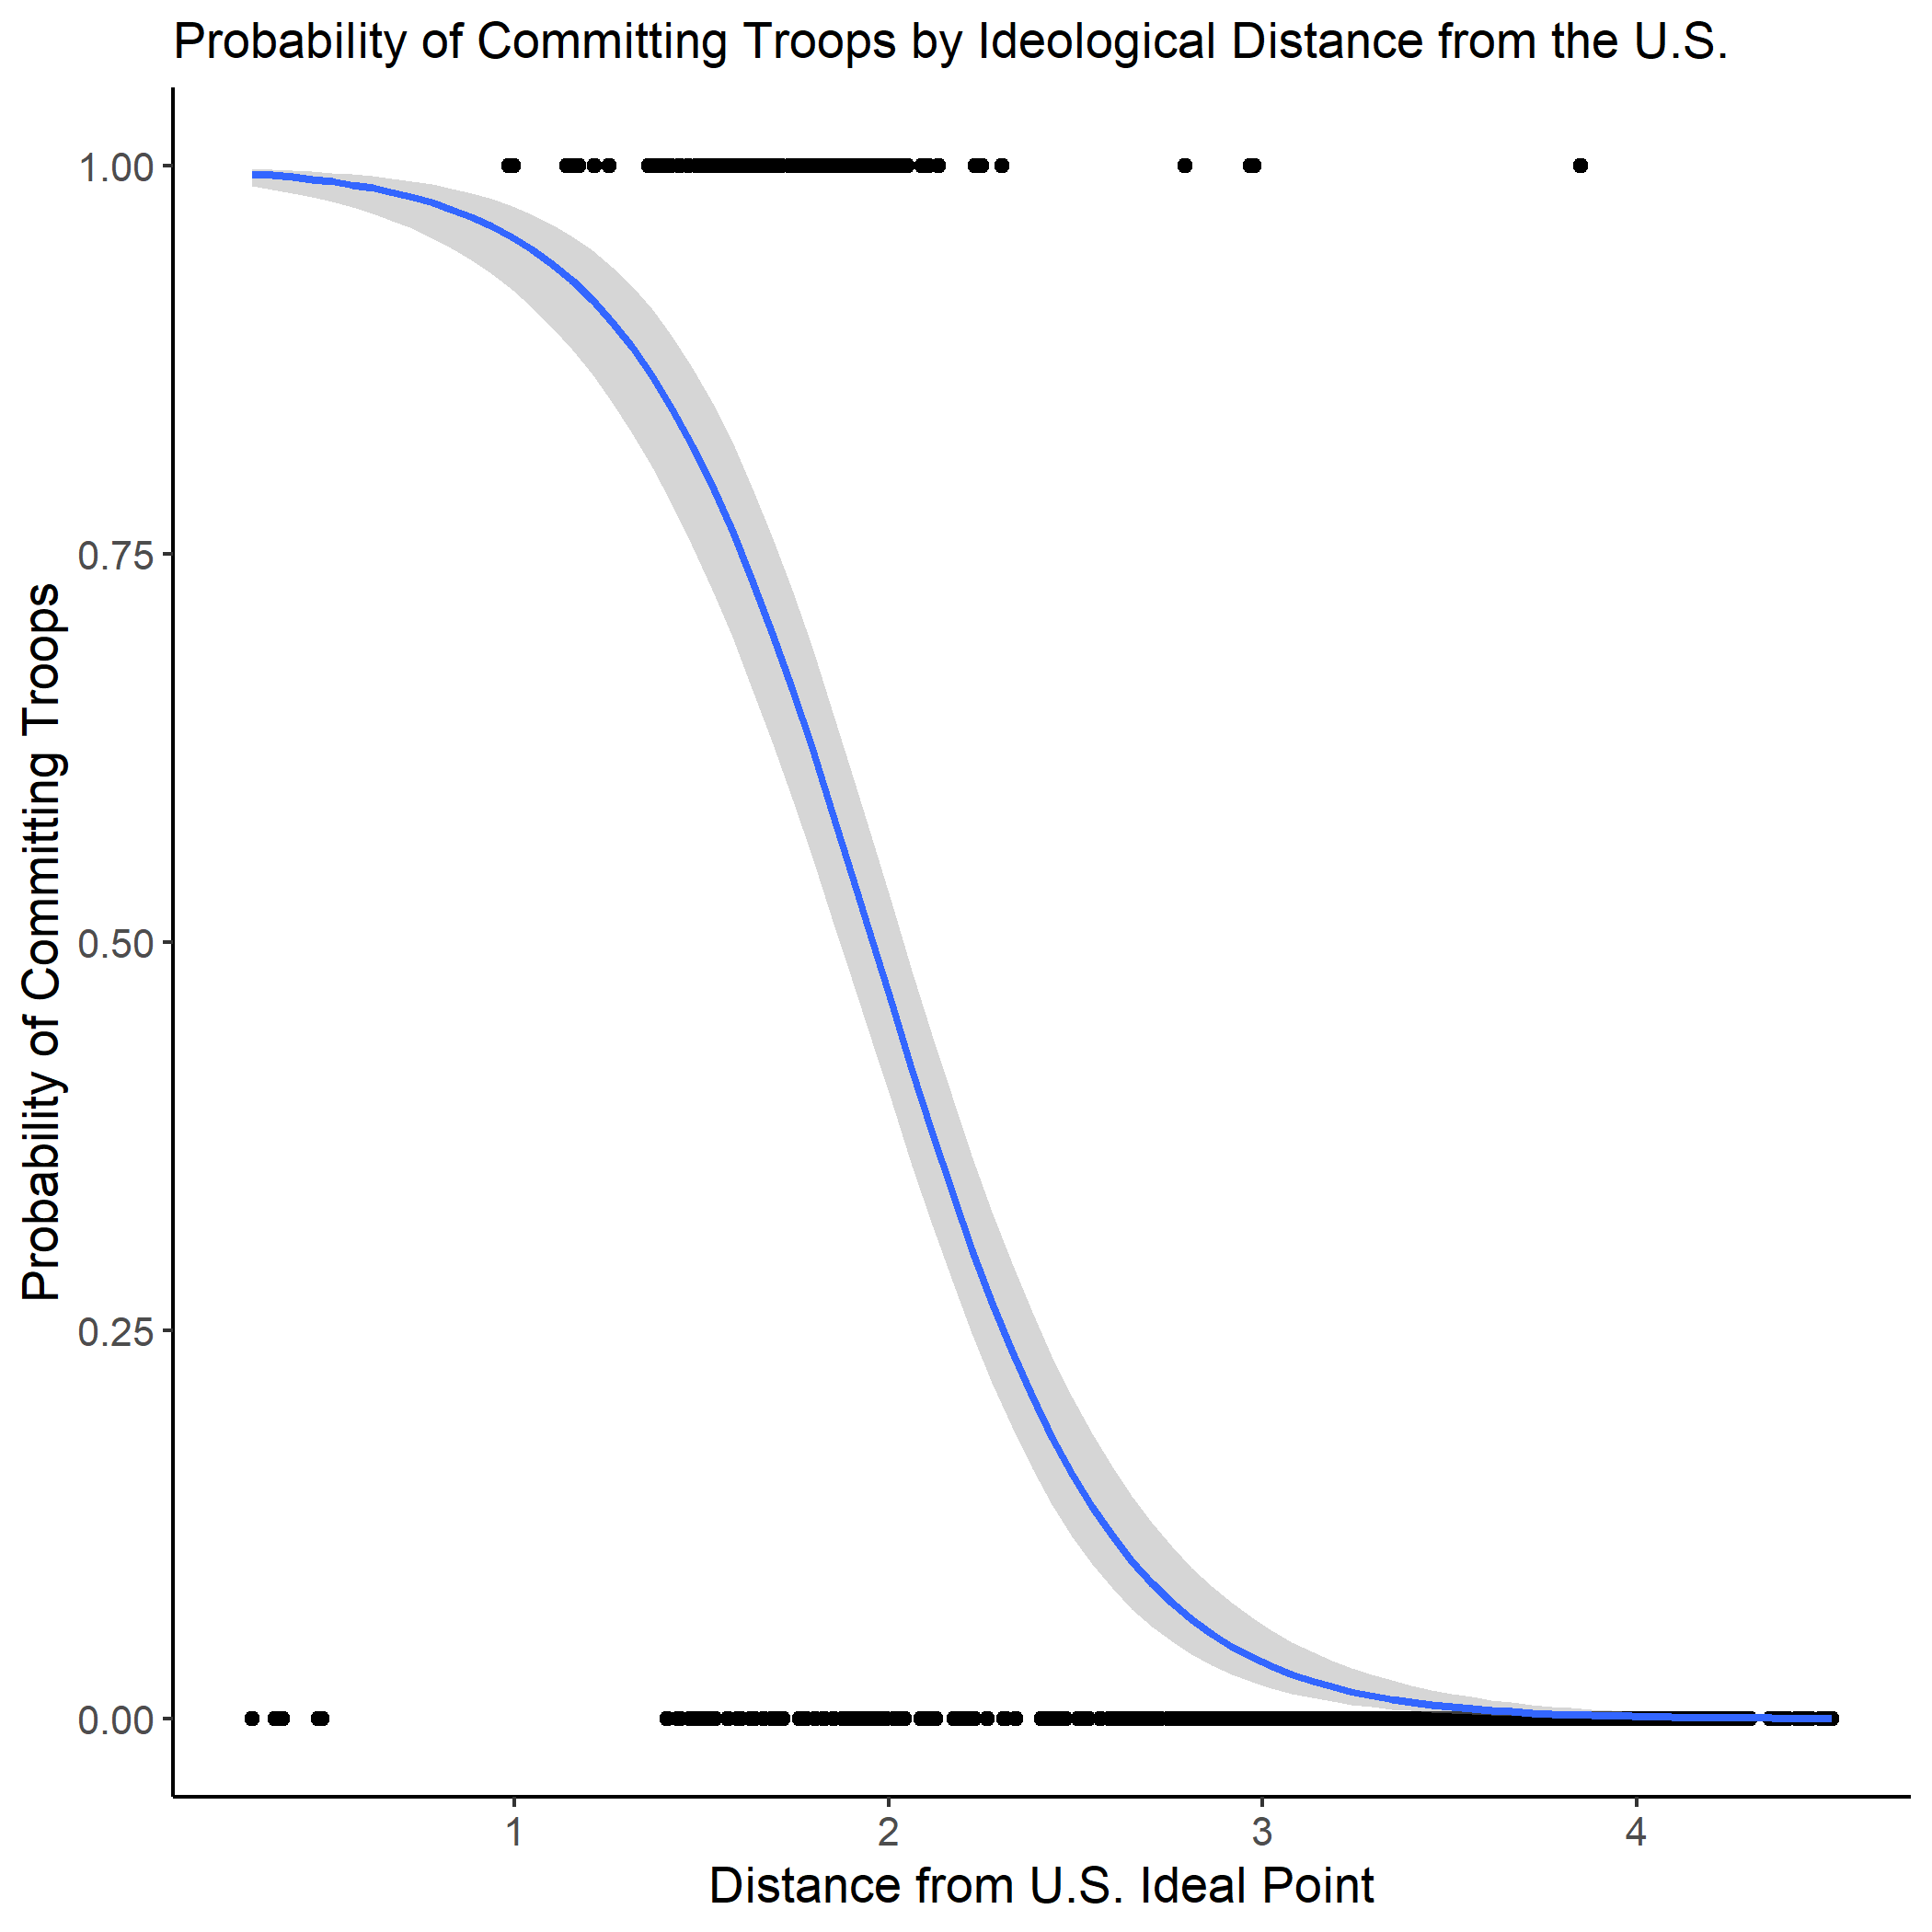
\includegraphics[scale=0.45]{../figures/logit.png}
\end{frame}

\begin{frame}{Number of Contributions}

  \begin{itemize}
    \item This is a bit tricky, because we are testing a non-linear hypothesis.
    \item Polynomial terms force a certain shape. We instead estimate a generalized additive model (GAM):
  \end{itemize}

  \begin{equation*}
    y_i = \alpha + f_1(x_1) + f_2(x_2) + ... + f_n(x_n) + \varepsilon_i
  \end{equation*}

\end{frame}

\begin{frame}{GAM -- No Canada}
  \centering
  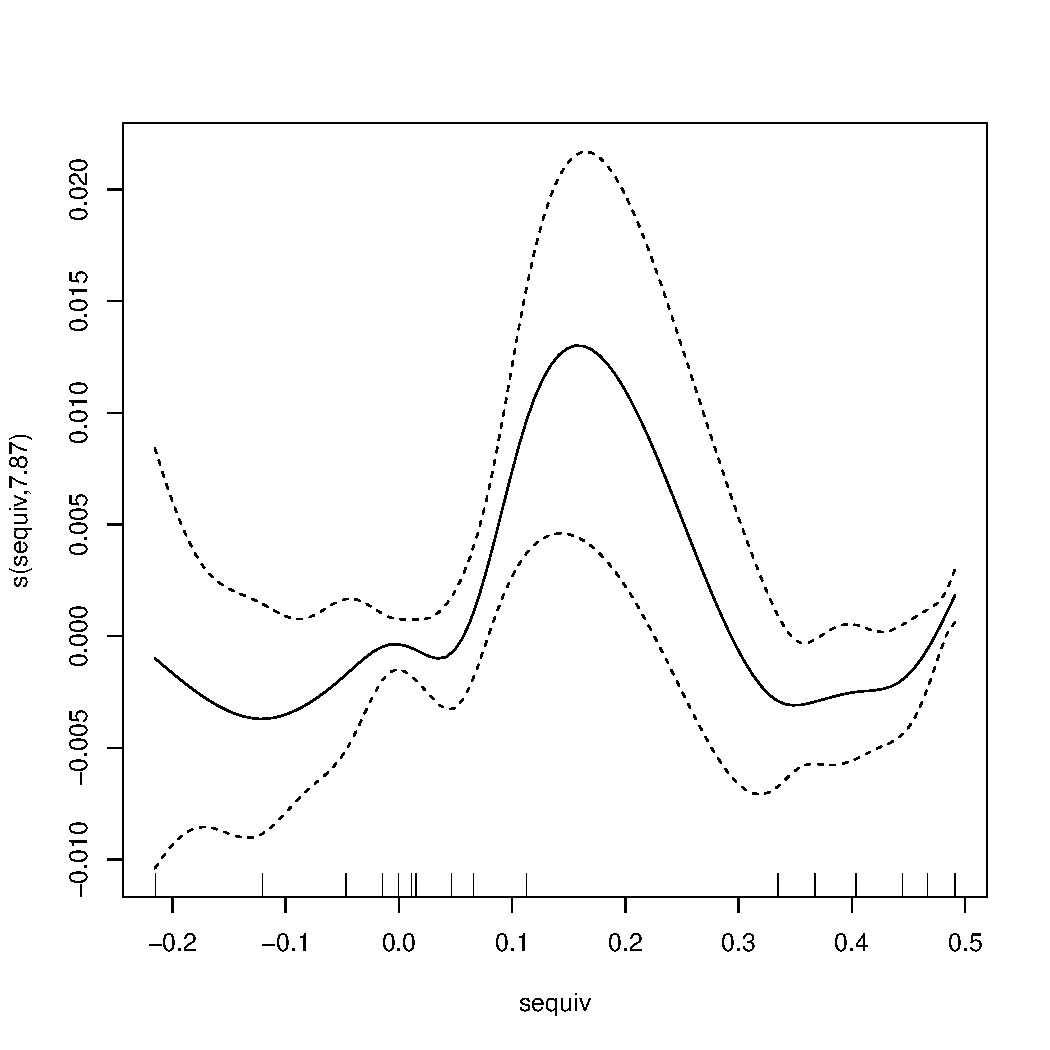
\includegraphics[scale=0.5]{../figures/no_can_gam.pdf}
\end{frame}

\begin{frame}{GAM -- With Canada}
  \centering
    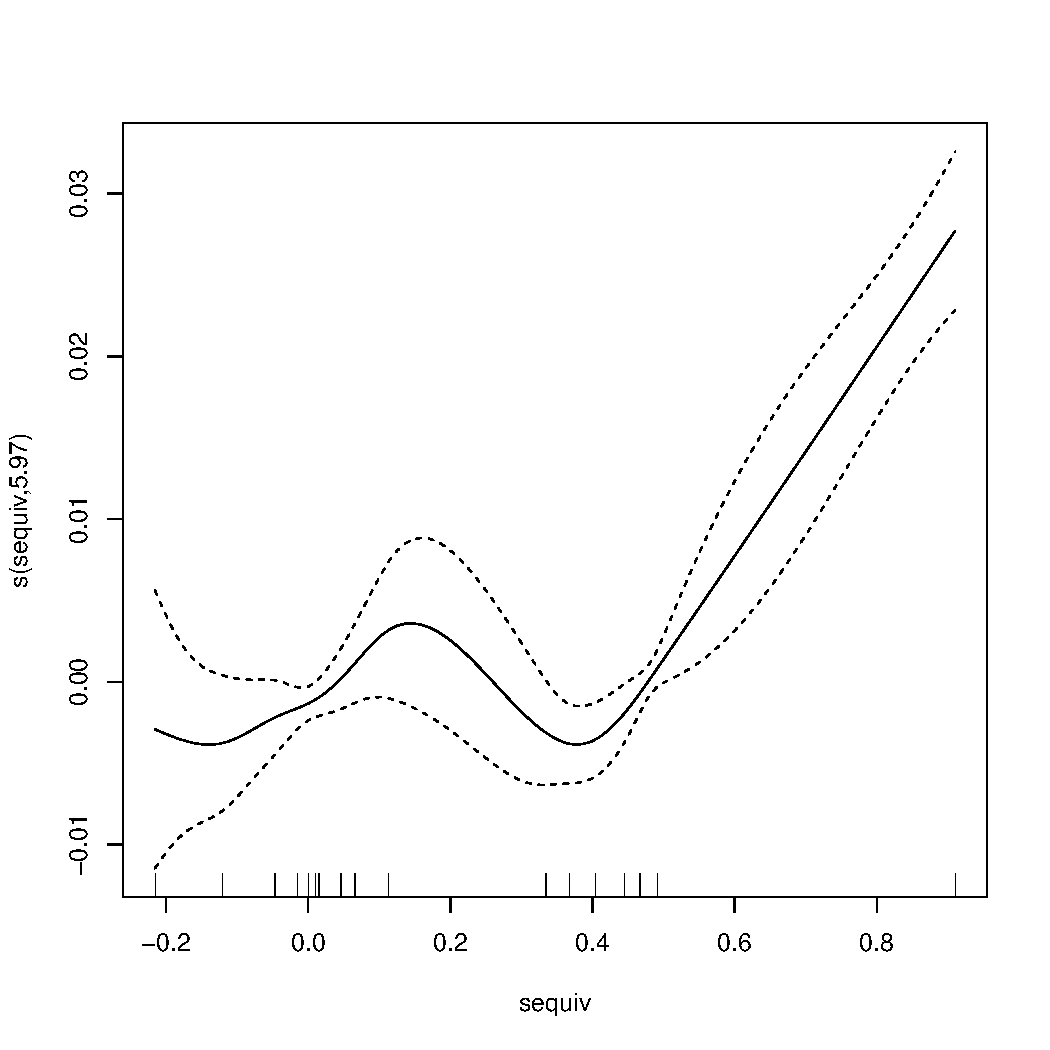
\includegraphics[scale=0.5]{../figures/can_gam.pdf}
\end{frame}


\begin{frame}{Recognized by Over-Contributor}
``...good opportunity for the New Zealand Defense Force to test its interoperability with contributing NATO nations. This deployment is an example of New Zealand's \textit{commitment to playing our part in supporting NATO in areas of common interest}.'' - Jonathan Coleman, New Zealand Defense Minister (2014)
\end{frame}

\begin{frame}{Recognized by the US}
``In the Libya operation, Norway and Denmark, have provided 12 percent of allied strike aircraft yet have struck about one third of the targets...These countries have, \textit{with their constrained resources}, found ways to do the training, buy the equipment, and field the platforms necessary to make a \textit{credible military contribution}.'' - US Defense Secretary Robert Gates (2011)
\end{frame}

\begin{frame}{Conclusion and Next Steps}
  \begin{itemize}
    \item Most reliable allies are those with potential to gain stronger ties, not those already closely aligned.
    \item Once final model is settled upon for Afghanistan, estimate the exact same model with Iraq data to see if the captured trend holds.
    \item Concerns:
    \begin{itemize}
      \item Structural equivalence -- Netherlands and Luxembourg have the same score as the UK.
      \item Canada as an outlier -- changing measure of tightness won't solve this. Just treat as unique and explain?
      \item GAM vs Polynomial
      \item Just control for casualties?
    \end{itemize}
  \end{itemize}
\end{frame}

\end{document}
